\documentclass[pdflatex,compress,mathserif]{beamer}

%\usetheme[dark,framenumber,totalframenumber]{ElektroITK}
\usetheme[darktitle,framenumber,totalframenumber]{ElektroITK}

\usepackage[utf8]{inputenc}
\usepackage[T1]{fontenc}
\usepackage{lmodern}
\usepackage[bahasai]{babel}
\usepackage{amsmath}
\usepackage{amsfonts}
\usepackage{amssymb}
\usepackage{graphicx}
\usepackage{multicol}
\usepackage{lipsum}

\newcommand*{\Scale}[2][4]{\scalebox{#1}{$#2$}}%

\title{PEMODELAN JARINGAN KOMUNIKASI}
\subtitle{Cisco Device Functions}

\author{Tim Dosen Pengampu}

\begin{document}

\maketitle

\section{Switches vs Hubs}

\begin{frame}
	\frametitle{Hubs and Switches}
	\begin{itemize}
		\item Hubs and switches perform a similar function.
		\item End hosts in a Local Area Network such as PCs, servers and printers plug into them with an Ethernet cable.
		\item The end hosts can then communicate with each other through the hub or switch.
	\end{itemize}
	\begin{center}
		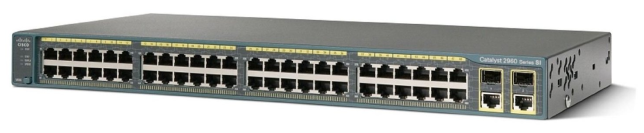
\includegraphics[width=0.6\linewidth]{img/img01}
	\end{center}
\end{frame}

\begin{frame}{Hubs and Switches}
	\begin{center}
		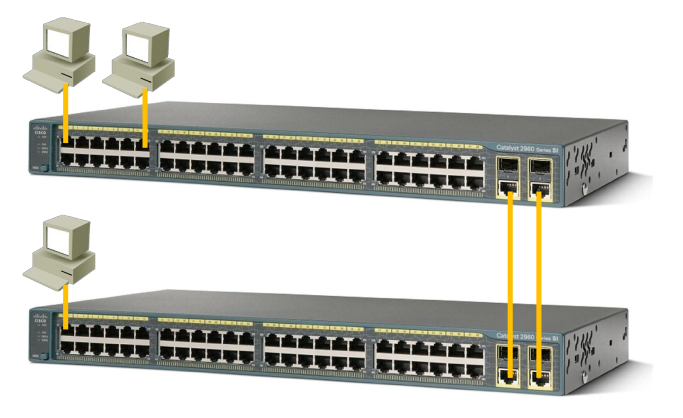
\includegraphics[width=0.7\linewidth]{img/img02}
	\end{center}
\end{frame}

\begin{frame}
	\frametitle{Hubs – Half-Duplex and Shared Collision Domain}
	\begin{itemize}
		\item Hubs operate in \textbf{half-duplex} mode.
		\item Attached hosts cannot send and receive data at the same time, they can only do one or the other.
		\item All hosts share the same \textbf{collision domain} - only one device can transmit at a time.
		\item If two hosts send at the same time a collision will occur.
		\item Hosts use Carrier-Sense Multiple Access with Collision Detection (CSMA/CD) to detect collisions and resend.
	\end{itemize}
\end{frame}

\begin{frame}
	\frametitle{Switches - Full-Duplex and Separate Collision Domains}
	\begin{itemize}
		\item Switches can operate in either \textbf{full-duplex} or \textbf{half-duplex} mode.
		\item In practice they always operate as full-duplex.
		\item Attached hosts can both send and receive data at the same time.
		\item All hosts have their own dedicated \textbf{collision domain}.
		Collision Detection is not required.
	\end{itemize}
\end{frame}

\begin{frame}
	\frametitle{Cisco Device Functions}
	\begin{center}
		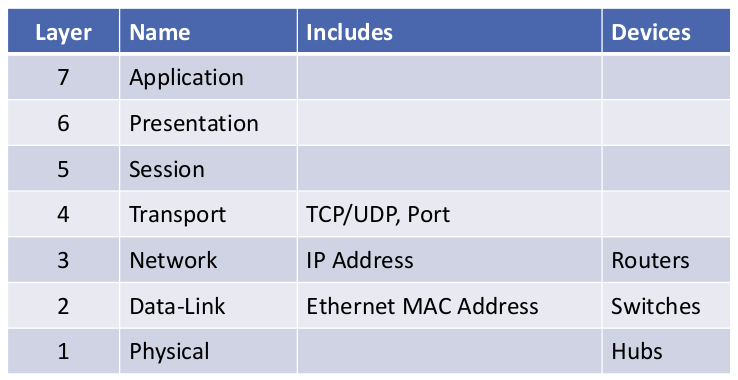
\includegraphics[width=0.7\linewidth]{img/img03}
	\end{center}
\end{frame}

\begin{frame}
	\frametitle{Hubs operate at OSI Layer 1}
	\begin{itemize}
		\item Hubs operate at Layer 1 of the OSI model.
		\item They are not MAC address aware.
		\item Whenever a frame is received it is flooded out all ports apart from the one it was received on.
		\item All attached hosts must process all packets.
	\end{itemize}
\end{frame}

\begin{frame}
	\frametitle{Switches operate at OSI Layer 2}
	\begin{itemize}
		\item Switches operate at Layer 2 of the OSI model.
		\item (They also operate at Layer 1.)
		\item They are MAC address aware.
	\end{itemize}
\end{frame}

\begin{frame}{Switches operate at OSI Layer 2}
	\begin{itemize}
		\item Whenever a frame is received the switch will look at the source MAC address in the Layer 2 Ethernet header.
		\item The learned MAC address will be added to the switch’s MAC address table, which maps MAC addresses to ports.
		\item If a unicast frame is later received with a known MAC address as the destination, the switch will send the frame out only the relevant port.
		\item This is better for performance and security as frames only go where they are required.
		\item Whenever a frame is received for the broadcast address or an unknown unicast destination (because the switch hasn’t learned the MAC address yet) it will be flooded out all ports apart from the one it was received on.
	\end{itemize}
\end{frame}

\section{Switch Operation}



\end{document}
